\section{Characters}

\subsection{B.A.D. Eleven}
Copy in everything of Eleven, BAD Eleven (Biological Altered Demon \#011, Elby) initially shares with her physical appearance, memories and attitudes.
However, during the course of the story, it will be increasingly evident that, unlike the original, Elby cannot manage her emotions, for example by transforming "her" love for Mike and the desire to see him again in pure obsession. This will lead her to be apathetic and unscrupulous, ready to eliminate any obstacle between her and her escape.\\
She has the same telekinetic prowess as Eleven, but the side effect is greatly reduced and the development of her ability is clearly superior, probably due to the influence of the Upside-Down and her origins.

\subsubsection{Circumplex}
\begin{center}
	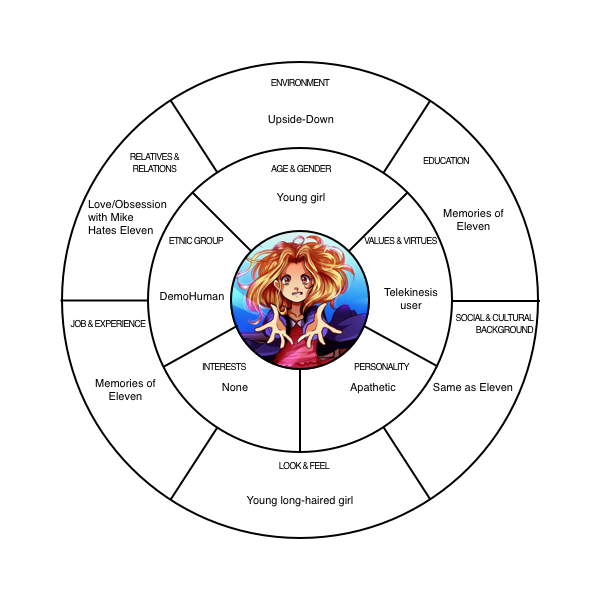
\includegraphics[width=0.76\linewidth]{images/graphs/characters/bad_eleven_circumplex.png}
	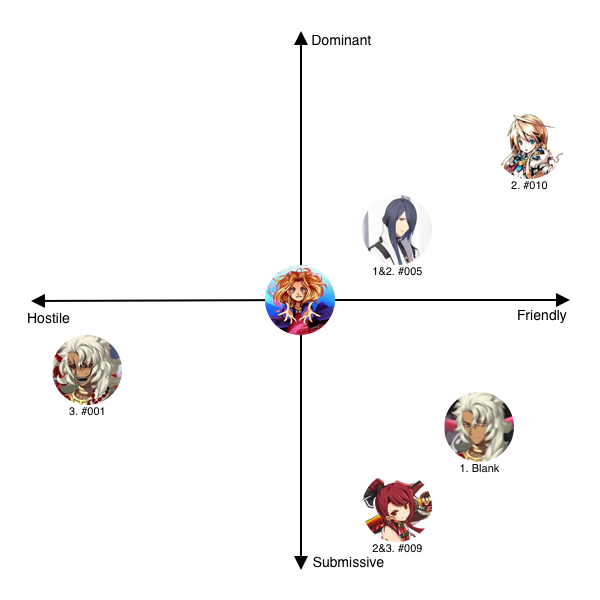
\includegraphics[width=0.76\linewidth]{images/graphs/characters/bad_eleven_map_of_relations.png}
\end{center}

\subsection{Kyle}
Kyle, alias \#001, is the first experimental subject of the MKUltra project. He's a 29-year-old boy, trapped in the Upside-Down since he was 15.
Despite the friendly and gentle attitude, the long period spent in darkness and solitude has greatly affected his mental stability, making him bipolar 
and easily irritated. Since birth he has the mental ability of biocynesis, the control and manipulation over organic matter. This ability applied to the 
Upside-Down allows him to control the ramifications of the Upside-Down Core, on condition that he is quite far from it.
His goal is to return home, not in the present time, but when he was kidnapped for experimentation, so that he could regain life and happiness denied to him.
To do this he requires the temporal ability of the Core and Elby's telecynesis to open the gap.
His personality changes drastically after discovering that, due to the laws of the multiverse, his plan is destined to fail. It therefore becomes extremely violent and sadistic, not even sparing the other numbers, which he believes are destined to suffer and need to be released through death. Moreover, he decides
 to transport the Core in various dimensions, in order to expand the Upside-Down and make all the inhabitants of the alternate realities suffer the same torture imposed on him.

\subsubsection{Backstory}
Born in a quiet Texas town, Kyle lives a happy and carefree life with his family. At the age of 6 he began to show the first signs of biocynesis, succeeding in bringing back a withered flower. Initially the use of his ability caused him violent migraines, but the more years passed and he became stronger, the less the side effects were intense. Although his ability had been kept as secret as possible, at the age of 12 he was tracked down by Brenner and, after witnessing the massacre of his family, he was imprisoned in an experimentation facility. In addition to continuous blood withdrawals, necessary for the creation of a serum to be used for the artificial production of test subjects, he was forced to use the biocynesis for war purposes, until the day when, exceeding the limit of his ability to attempt a escape, he was wrapped in a black cloud and disappeared.

\subsubsection{Circumplex}
\begin{center}
	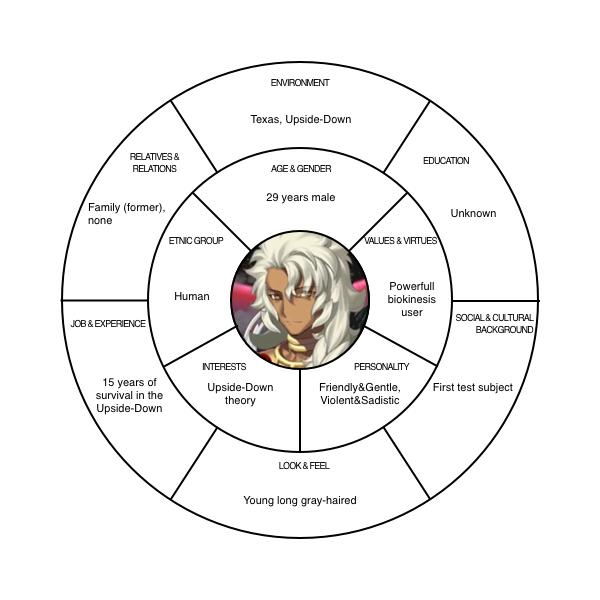
\includegraphics[width=0.76\linewidth]{images/graphs/characters/kyle_circumplex.png}
	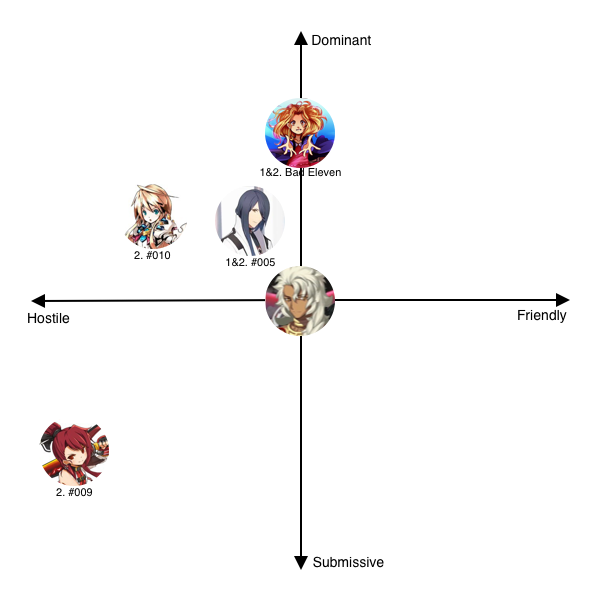
\includegraphics[width=0.76\linewidth]{images/graphs/characters/kyle_map_of_relations.png}
	
\includegraphics[width=0.76\linewidth]{images/graphs/characters/001_map_of_relations.png}
\end{center}

\subsection{Minor characters}

\subsubsection{\#005}
A shut-in, he doesn't like be with others.\\
He has the Mental Synchronization Kinesis, the ability to control beasts, with the condition of them being weaker than him.

\subsubsection{\#009}
Self proclaimed Queen of the Upside-Down, she is a very strong and passionate girl.\\
Her prowess is the Pyrokinesis, the ability to accelerate atoms and create fire.\\
She is extremely protective towards her little twin brother \#010.

\subsubsection{\#010}
A very shy guy, always hiding in the shadow of her older twin sister \#009.\\
He has the Cryokinesis, the ability to slow atoms freeze things.
